\apendice{Documentación de usuario}

\section{Introducción}
En esta sección se presenta la documentación completa de usuario para ReservApp, un sistema integral de gestión de reservas desarrollado con tecnología Java Spring Boot. ReservApp está diseñado para facilitar la administración y reserva de establecimientos, proporcionando una plataforma intuitiva tanto para usuarios finales como para administradores del sistema.

El sistema permite a los usuarios realizar reservas en establecimientos asignados, gestionar convocatorias de reuniones y administrar sus perfiles personales. Los administradores pueden gestionar usuarios, establecimientos, perfiles del sistema y supervisar todas las reservas realizadas.

Esta documentación está estructurada para guiar al usuario paso a paso a través de todas las funcionalidades disponibles, desde el registro inicial hasta las operaciones más avanzadas de administración del sistema.

\section{Requisitos de usuarios}
El acceso a la aplicación está condicionado únicamente a la disponibilidad de una conexión a internet, dado su diseño como plataforma web. Esto garantiza una total compatibilidad multiplataforma, permitiendo su uso desde dispositivos móviles, tabletas y ordenadores. No obstante, para optimizar la experiencia de usuario, se aconseja el acceso desde un ordenador.

\section{Instalación}
Dado que se trata de una aplicación web, no es necesaria ninguna instalación local. Se puede acceder a la aplicación de forma inmediata a través del enlace \url{https://reservapp-1u8c.onrender.com/}.

\section{Manual del usuario}
A continuación se detallan las operaciones que se pueden realizar en la aplicación.

\subsection{Acceso a la Aplicación}

\begin{figure}[H]
	\centering
		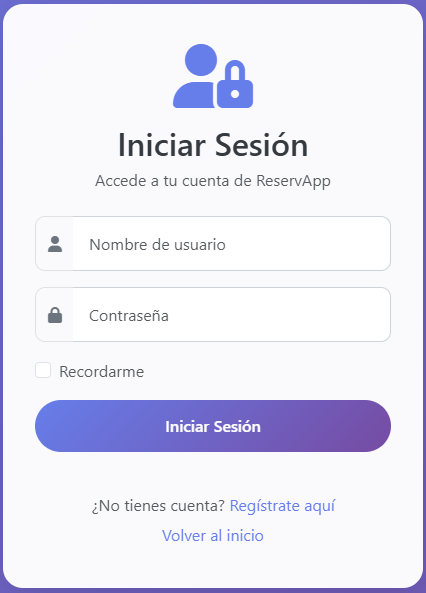
\includegraphics[width=0.5\linewidth]{reservapp_login}
	\caption{Página inicial de la aplicación.}
	\label{fig:reservapp_login}
\end{figure}

\subsubsection{Registro de un nuevo usuario}
Nada más acceder a la aplicación, se mostrará por defecto la página de inicio, tal y como se puede ver en la figura ~\ref{fig:reservapp_login}. Si es la primera vez que se accede a la aplicación, será necesario crear una cuenta para poder acceder a las funcionalidades de reserva. Estos son los pasos a seguir:

\begin{enumerate}
   \item \textbf{Acceder a la página de registro}:

   \begin{itemize}
      \item Desde la página de inicio, hacer clic en ``Regístrate aquí''.
      \item O navegar directamente a ``/registro''.
   \end{itemize}
   \item \textbf{Completar el formulario de registro}:
   \begin{itemize}

      \begin{figure}[H]
         \centering
         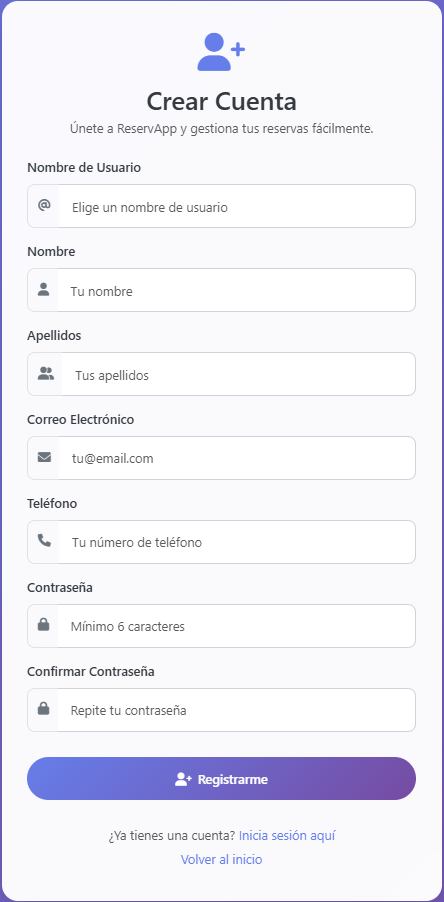
\includegraphics[width=0.5\linewidth]{reservapp_registro}
         \caption{Página para el registro de usuario.}
         \label{fig:reservapp_registro}
      \end{figure}

      \item Al acceder, se mostrará una página como se muestra en la figura ~\ref{fig:reservapp_registro}.
      \item \textbf{Nombre de Usuario (ID de Usuario)}: Introducir un identificador único de 3-10 caracteres alfanuméricos (sin espacios ni símbolos especiales).
      \item \textbf{Nombre}: Introducir el nombre (máximo 50 caracteres).
      \item \textbf{Apellidos}: Introducir los apellidos (máximo 50 caracteres).
      \item \textbf{Correo Electrónico}: Introducir una dirección de email válida y única.
      \item \textbf{Teléfono}: Introducir número de teléfono (5-12 caracteres).
      \item \textbf{Contraseña}: Crear una contraseña segura.
      \item \textbf{Confirmar Contraseña}: Repetir la contraseña para verificación.
   \end{itemize}
   \item \textbf{Enviar el formulario}:
   \begin{itemize}
      \item Hacer clic en ``Registrarse''.
      \item El sistema validará los datos y creará la cuenta.
      \item Se mostrará un mensaje de confirmación.
   \end{itemize}
\end{enumerate}

\textbf{Notas importantes}:
\begin{itemize}
   \item El ID de usuario y el correo electrónico deben ser únicos en el sistema.
   \item Todos los campos son obligatorios.
   \item El sistema \emph{hashea} automáticamente las contraseñas.
\end{itemize}

\subsubsection{Inicio de sesión (login)}
En caso de tener un usuario previamente creado se podrá acceder a la aplicación, a través de la página de inicio, tal y como se muestra en la figura~\ref{fig:reservapp_login}, con las credenciales existentes. Estos son los pasos a seguir:

\begin{enumerate}
   \item \textbf{Acceder a la página de login}:

   \begin{itemize}
      \item Navegar a /login o hacer clic en ``Iniciar Sesión''.
   \end{itemize}
   \item \textbf{Introducir credenciales}:
   \begin{itemize}
      \item \textbf{Usuario}: Introducir el ID de usuario registrado.
      \item \textbf{Contraseña}: Introducir la contraseña correspondiente.
      \item Opcionalmente, marcar ``Recordarme'' para mantener la sesión activa.
   \end{itemize}
   \item \textbf{Iniciar sesión}:
   \begin{itemize}
      \item Hacer clic en ``Iniciar Sesión''.
      \item El sistema redirigirá al menú principal tras la autenticación exitosa.
   \end{itemize}
\end{enumerate}

\textbf{Mensajes de error comunes}:
\begin{itemize}
   \item ``Usuario o contraseña incorrectos'': Verificar las credenciales introducidas.
   \item Usuario bloqueado: Contactar con el administrador del sistema.
\end{itemize}

\subsubsection{Cierre de Sesión}
Pulsando el botón de ``Cerrar Sesión'', provocará el cierre de la sesión actual de forma segura. Estos son los pasos a seguir:

\begin{enumerate}
   \item Desde cualquier página del sistema, hacer clic en el botón ``Cerrar Sesión'' en la sección superior.
   \item El sistema cerrará la sesión y redirigirá a la página de login.
\end{enumerate}

\newpage

\subsection{Navegación Principal}

\subsubsection{Menú Principal}
El menú principal es el centro de control del sistema, organizado en secciones según el rol del usuario.

\begin{figure}[H]
	\centering
		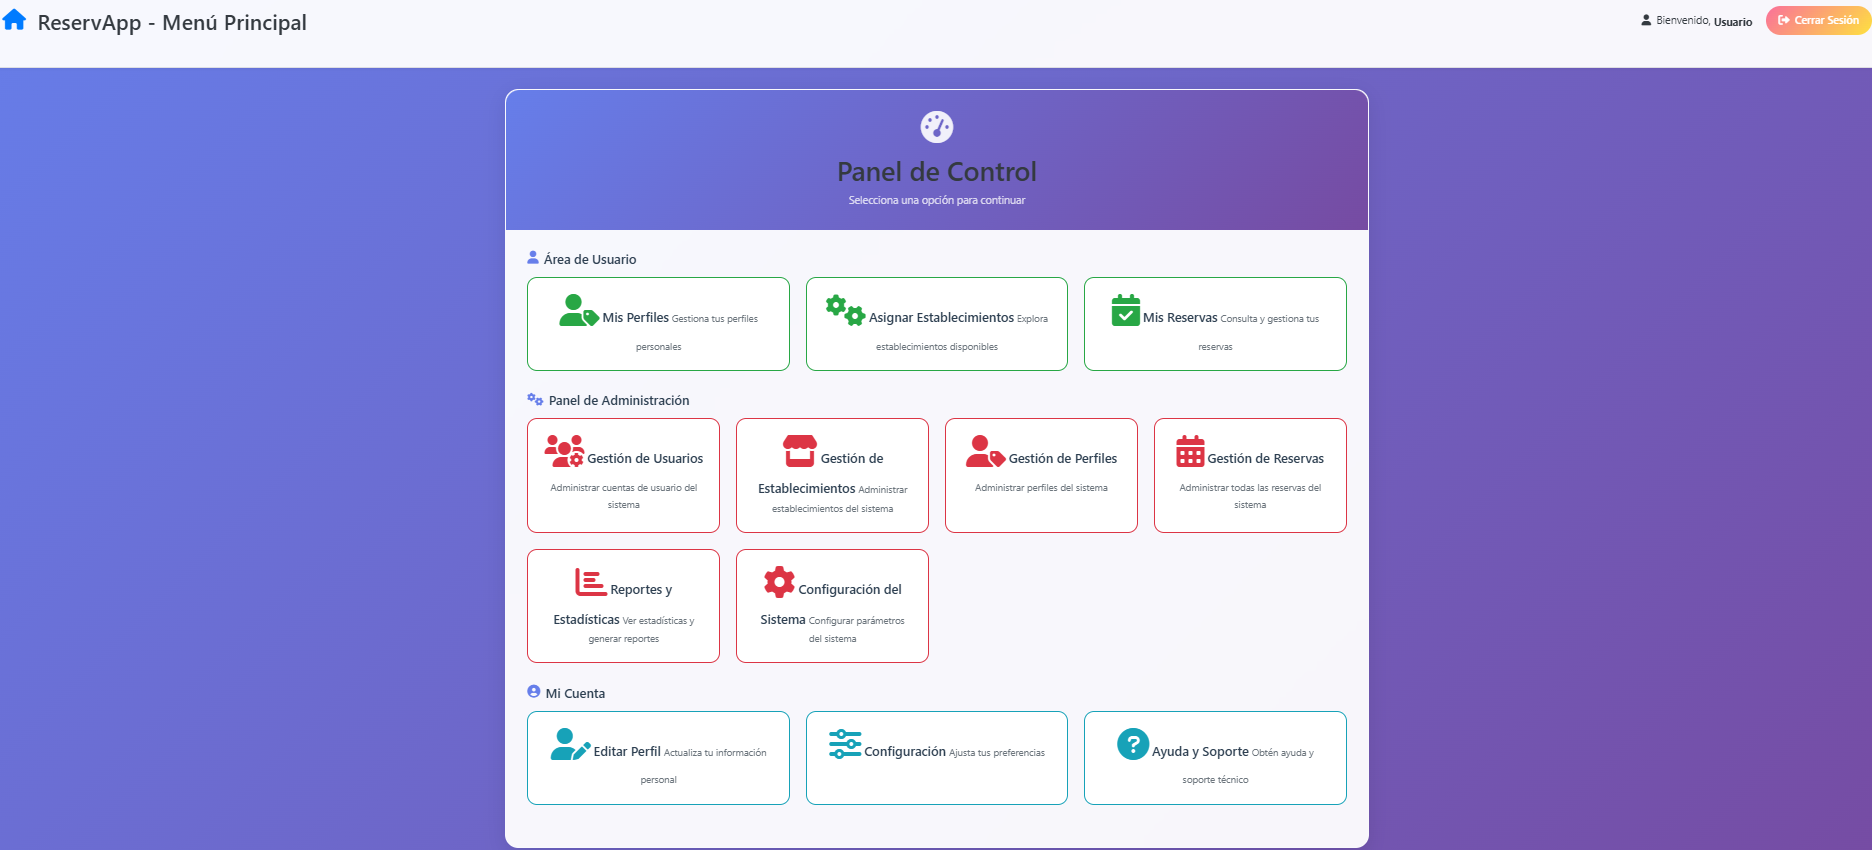
\includegraphics[width=1.0\linewidth]{reservapp_menu_principal_admin}
	\caption{Menú Principal para usuario administrador.}
	\label{fig:reservapp_menu_principal_admin}
\end{figure}

\begin{figure}[H]
	\centering
		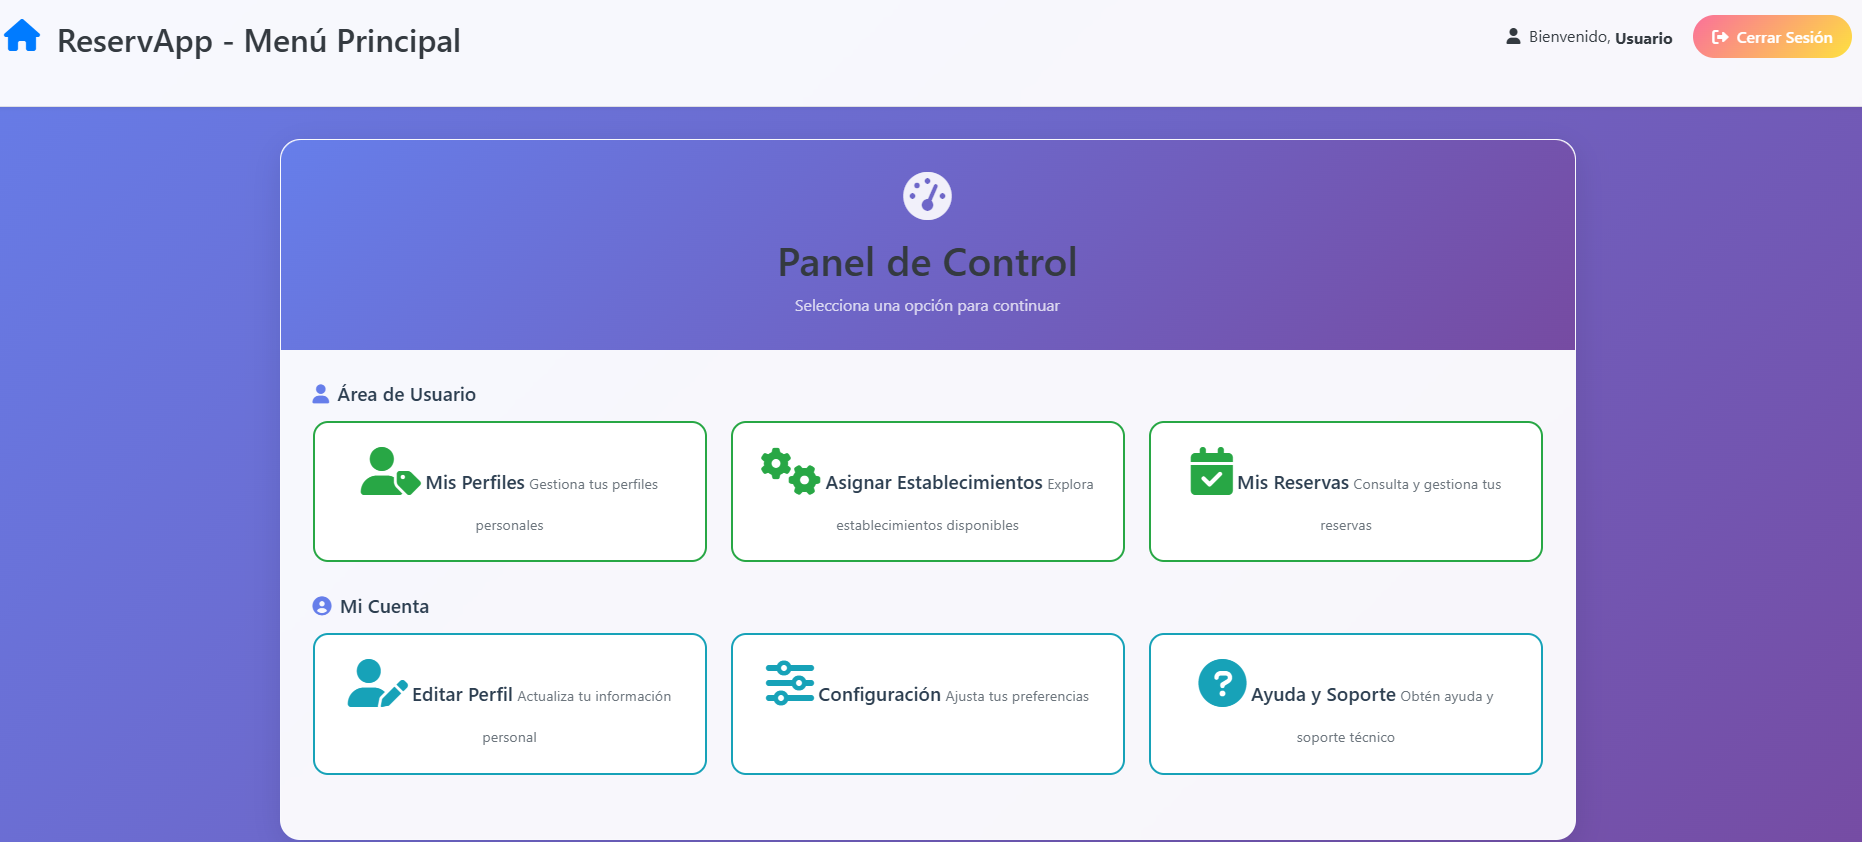
\includegraphics[width=1.0\linewidth]{reservapp_menu_principal_no_admin}
	\caption{Menú Principal para usuario no administrador.}
	\label{fig:reservapp_menu_principal_no_admin}
\end{figure}

\begin{itemize}
   \item Para todos los usuarios, tal y como se muestra en la figura~\ref{fig:reservapp_menu_principal_no_admin}, aparecen disponibles las siguientes secciones:
   \begin{itemize}
      \item \textbf{Área de Usuario}:
      \begin{itemize}
         \item Mis Perfiles: Gestión de perfiles personales.
         \item Asignar Establecimientos: Explorar y solicitar acceso a establecimientos
         \item Mis Reservas: Consultar y gestionar reservas personales
      \end{itemize}
      \item \textbf{Mi Cuenta}:
      \begin{itemize}
         \item Editar Perfil: Actualizar información personal.
         \item Configuración: Ajustar preferencias del usuario.
         \item Ayuda y Soporte: Acceder a documentación y soporte.
      \end{itemize}
   \end{itemize}
   \item Para todos los usuarios que sean administradores, además de las opciones que se muestra para el resto de usuarios,  tal y como se muestra en la figura~\ref{fig:reservapp_menu_principal_admin}, aparecen disponibles las siguientes secciones:
   \begin{itemize}
      \item \textbf{Panel de Administración}:
      \begin{itemize}
         \item Gestión de Usuarios: Administrar cuentas de usuario.
         \item Gestión de Establecimientos: Administrar establecimientos del sistema.
         \item Gestión de Perfiles: Administrar perfiles del sistema.
         \item Gestión de Reservas: Supervisar todas las reservas.
         \item Reportes y Estadísticas: Ver estadísticas del sistema.
         \item Configuración del Sistema: Configurar parámetros globales.
      \end{itemize}
   \end{itemize}
\end{itemize}

\newpage

\subsection{Gestión de Reservas}

\subsubsection{Visualizar Mis Reservas}
Permite consultar los establecimientos disponibles para realizar reservas, tal y como se ilustra en la figura~\ref{fig:reservapp_mis_reservas}. Estos son los pasos a seguir:

\begin{figure}[H]
	\centering
		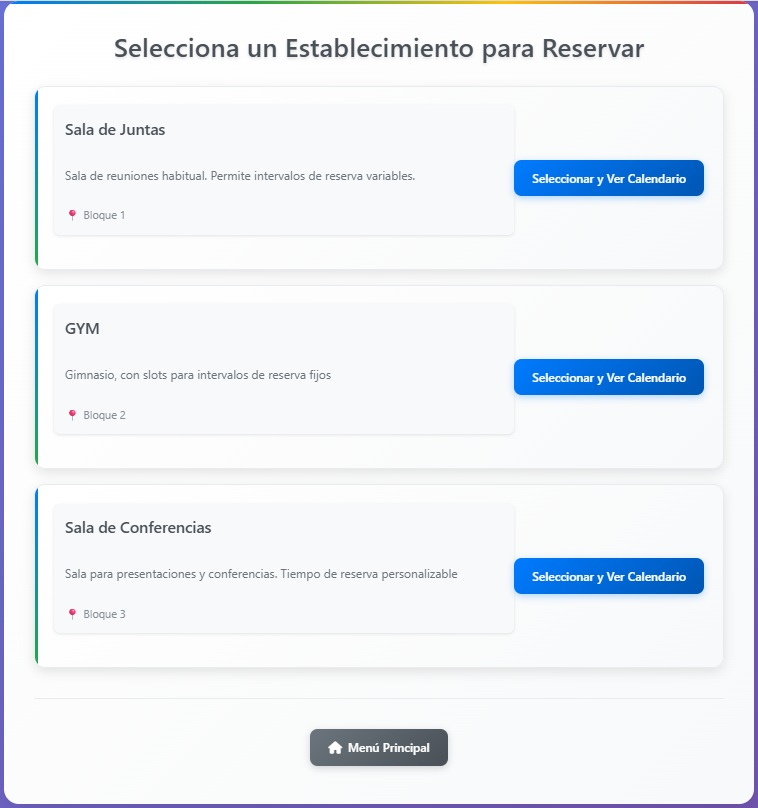
\includegraphics[width=0.75\linewidth]{reservapp_mis_reservas}
	\caption{Página de ``Mis Reservas'' donde se muestran los establecimientos asignados.}
	\label{fig:reservapp_mis_reservas}
\end{figure}

\begin{enumerate}
   \item \textbf{Acceder a ``Mis Reservas''}:
   \begin{itemize}
      \item Desde el menú principal, hacer clic en ``Mis Reservas''.
      \item O navegar directamente a /misreservas.
   \end{itemize}
   \item \textbf{Seleccionar establecimiento}:
   \begin{itemize}
      \item Se mostrará una lista de establecimientos asignados al usuario.
      \item Cada establecimiento muestra:
      \begin{itemize}
         \item Nombre del establecimiento.
         \item Descripción.
         \item Dirección.
      \end{itemize}
      \item Hacer clic en ``Seleccionar y Ver Calendario'' para el establecimiento deseado.
   \end{itemize}
\end{enumerate}

\newpage

\subsubsection{Crear Nueva Reserva}
Permite crear una nueva reserva para un establecimiento en concreto, después de haber seleccionado el establecimiento en la página como la que se ilustra en la figura~\ref{fig:reservapp_mis_reservas}. Estos son los pasos a seguir:

\begin{figure}[H]
	\centering
	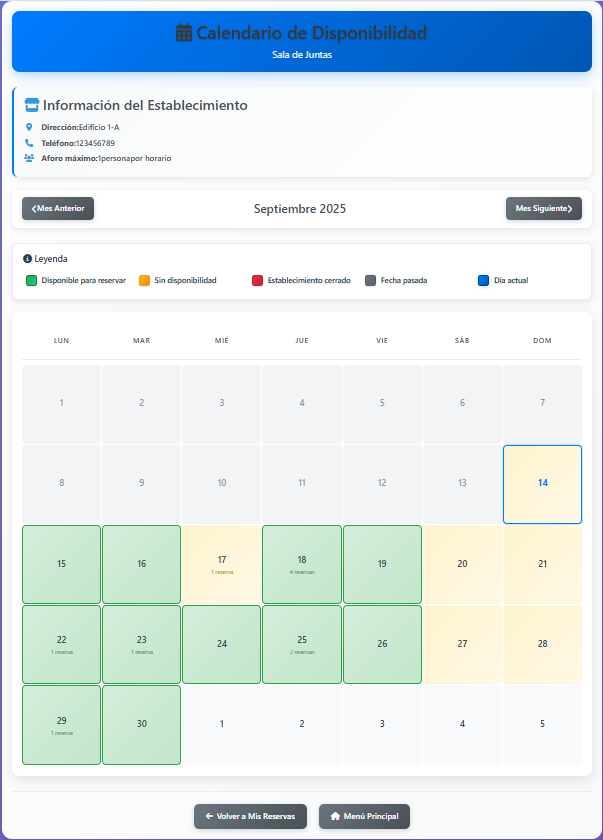
\includegraphics[width=0.85\linewidth]{reservapp_calendario}
	\caption{Página con el calendario del mes actual mostrando la disponibilidad.}
	\label{fig:reservapp_calendario}
\end{figure}

\begin{figure}[H]
	\centering
		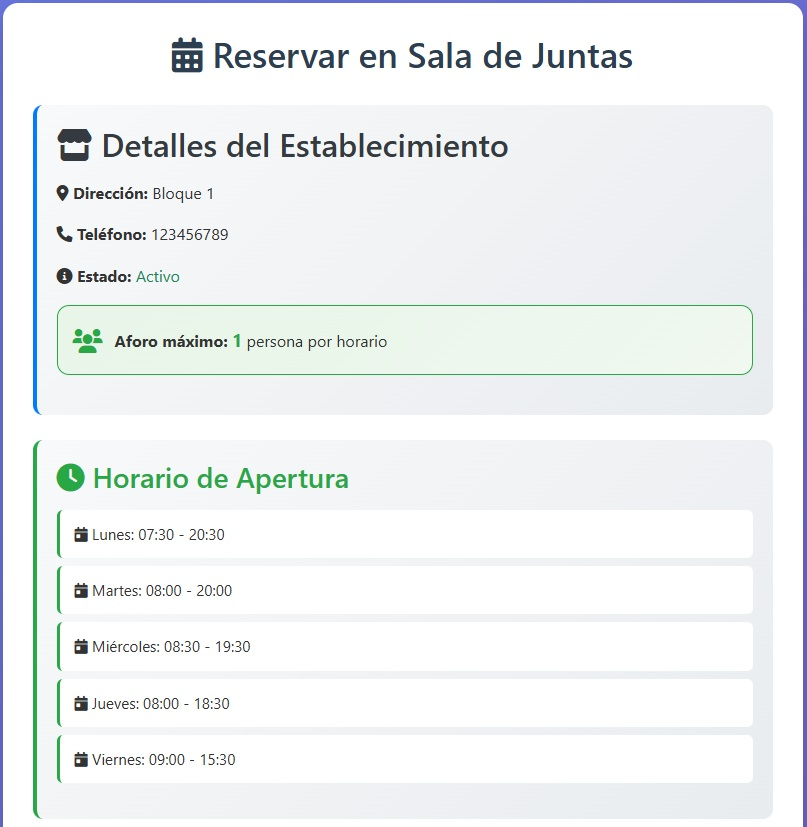
\includegraphics[width=0.5\linewidth]{reservapp_establecimiento_reserva}
	\caption{Página con la información del establecimiento y el régimen horario que tiene.}
	\label{fig:reservapp_establecimiento_reserva}
\end{figure}

\begin{enumerate}
   \item \textbf{Acceder al calendario de reservas}:
   \begin{itemize}
      \item Desde ``Mis Reservas'', seleccionar un establecimiento.
      \item Se muestra un calendario con el mes en curso con la disponibilidad de días para poder concretar una reserva, tal y como se muestra en la figura~\ref{fig:reservapp_calendario}.
   \end{itemize}
   \item \textbf{Seleccionar un día con disponibilidad}:
   \begin{itemize}
      \item Se mostrará la información del establecimiento con su régimen horario, tal y como se muestra en la figura~\ref{fig:reservapp_establecimiento_reserva}.
      \item \textbf{Detalles}: Dirección, teléfono, estado.
      \item \textbf{Aforo}: Número de reservas simultáneas o concurrentes.
      \item \textbf{Horarios de apertura}: Días y horas disponibles para reservas.
   \end{itemize}
   \item \textbf{Seleccionar fecha y hora}:
   \begin{itemize}
      \item \textbf{Fecha}: Seleccionar una fecha futura en el calendario.
      \item \textbf{Horario}: Dependiendo del establecimiento:
      \begin{itemize}
         \item \textbf{Slots predefinidos}: Seleccionar de una lista de horarios disponibles, tal y como se muestra en la figura~\ref{fig:reservapp_reserva_slot}.
         \item \textbf{Horario libre}: Permite escoger entre los periodos variables disponibles, tal y como se muestra en la figura~\ref{fig:reservapp_periodos}, o bien introducir hora de inicio y fin manualmente, tal y como se muestra en la figura~\ref{fig:reservapp_reserva}.
      \end{itemize}
   \end{itemize}

   \begin{figure}[H]
	\centering
		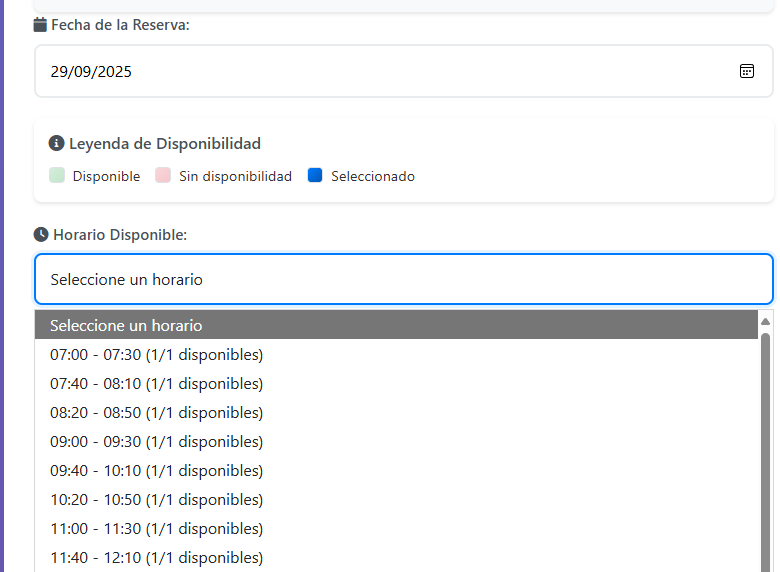
\includegraphics[width=0.5\linewidth]{reservapp_reserva_slot}
	\caption{Sección donde se introducen los datos de la reserva con duración fija.}
	\label{fig:reservapp_reserva_slot}
   \end{figure}

   \begin{figure}[H]
	\centering
	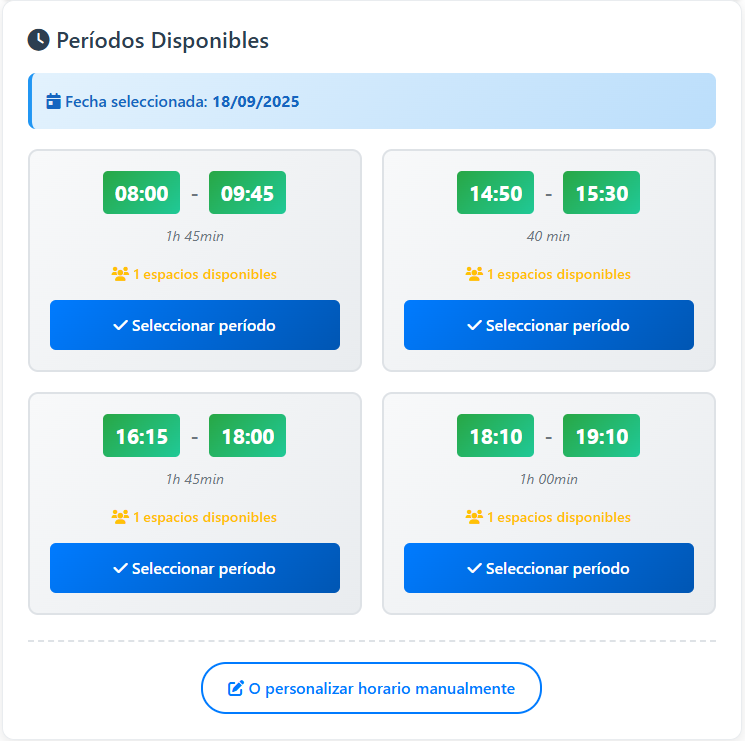
\includegraphics[width=0.5\linewidth]{reservapp_periodos}
	\caption{Sección donde se muestran los periodos variables disponibles.}
	\label{fig:reservapp_periodos}
\end{figure}

   \begin{figure}[H]
	\centering
		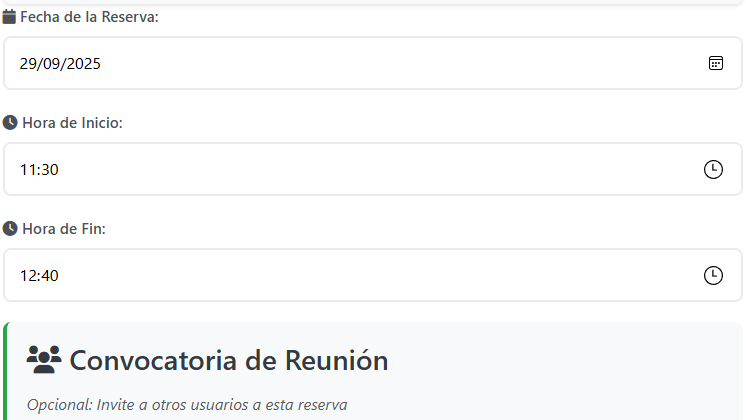
\includegraphics[width=0.5\linewidth]{reservapp_reserva}
	\caption{Sección donde se introducen los datos de la reserva con duración variable.}
	\label{fig:reservapp_reserva}
   \end{figure}

   \item \textbf{Configurar convocatoria (opcional)}:
   \begin{itemize}
      \item \textbf{Enlace de reunión}: Introducir URL de videoconferencia (Google Meet, Zoom, Teams, etc.).
      \item \textbf{Observaciones}: Añadir notas, agenda o temas a tratar.
      \item \textbf{Invitar usuarios}:
      \begin{itemize}
         \item Buscar usuarios por nombre, apellido, ID o email.
         \item Seleccionar usuarios de los resultados de búsqueda.
         \item Los usuarios seleccionados aparecerán en la lista de invitados.
      \end{itemize}
   \end{itemize}
   \item \textbf{Confirmar reserva}:
   \begin{itemize}
      \item Revisar todos los datos introducidos.
      \item Hacer clic en ``Confirmar Reserva''.
      \item El sistema validará la disponibilidad y creará la reserva.
      \item Se enviarán notificaciones por correo al usuario y a los invitados.
   \end{itemize}
\end{enumerate}

\textbf{Validaciones del sistema}:
\begin{itemize}
   \item La fecha debe ser futura.
   \item El horario debe estar dentro de las franjas de apertura del establecimiento.
   \item No debe exceder el aforo máximo del establecimiento.
   \item La hora de fin debe ser posterior a la hora de inicio
\end{itemize}

\subsubsection{Modificar una Reserva}
Permite modificar una reserva previamente creda para un establecimiento en concreto, tal y como se ilustra en la figura~\ref{fig:reservapp_editar_reserva}. Estos son los pasos a seguir:

\begin{figure}[H]
	\centering
		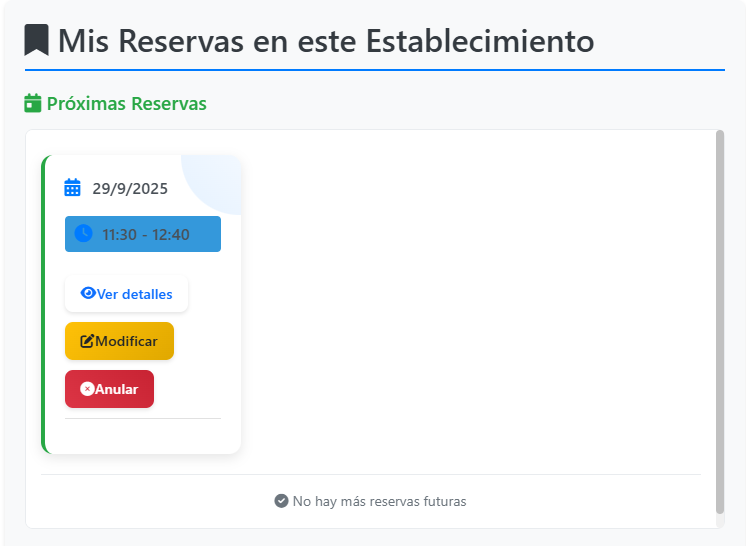
\includegraphics[width=0.5\linewidth]{reservapp_futuras_reservas}
	\caption{Vista del detalle de una reserva futura.}
	\label{fig:reservapp_futuras_reservas}
\end{figure}

\begin{figure}[H]
	\centering
		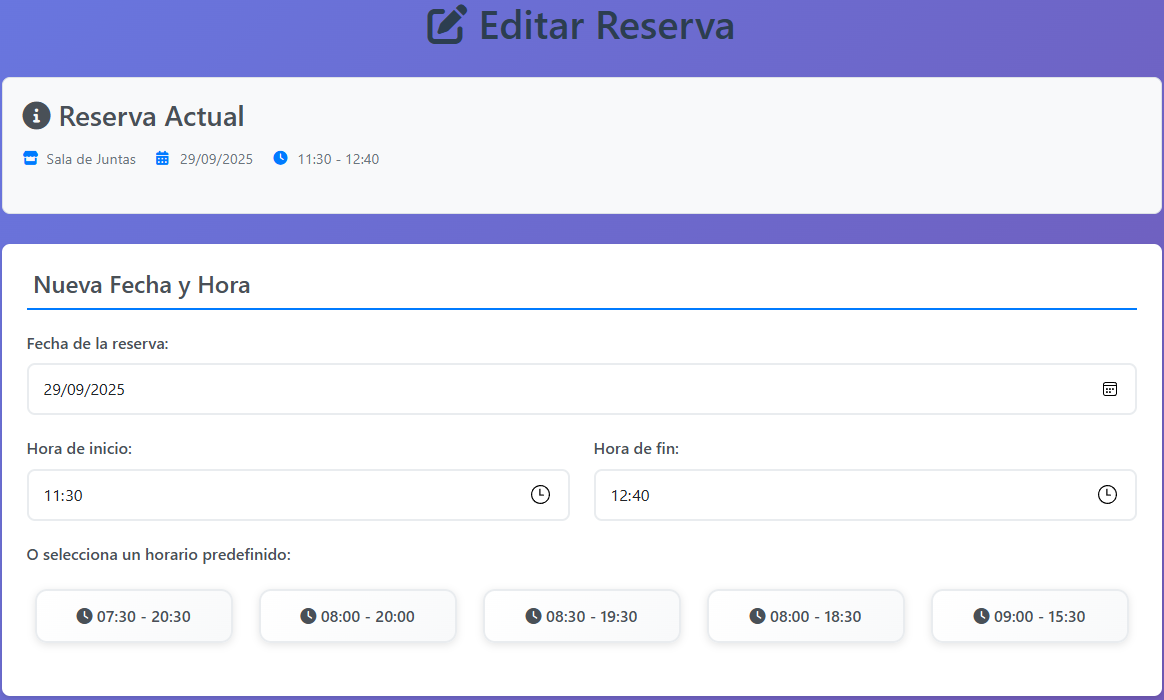
\includegraphics[width=0.5\linewidth]{reservapp_editar_reserva}
	\caption{Página que muestra los datos de la reserva para modificar.}
	\label{fig:reservapp_editar_reserva}
\end{figure}

\begin{enumerate}
   \item \textbf{Localizar la reserva}:
   \begin{itemize}
      \item Desde el calendario del establecimiento, buscar la reserva en ``Próximas Reservas''.
      \item Hacer clic en ``Modificar'' en la reserva deseada. Aparecerá como la imagen de la figura~\ref{fig:reservapp_futuras_reservas}.
   \end{itemize}
   \item \textbf{Editar datos de la reserva}:
   \begin{itemize}
      \item \textbf{Fecha y hora}: Cambiar según disponibilidad.
      \item \textbf{Convocatoria}: Modificar enlace, observaciones o lista de invitados.
      \item Todos los campos son editables siguiendo las mismas reglas que en la creación.
   \end{itemize}
   \item \textbf{Configurar convocatoria (opcional)}:
   \begin{itemize}
      \item \textbf{Enlace de reunión}: Introducir URL de videoconferencia (Google Meet, Zoom, Teams, etc.).
      \item \textbf{Observaciones}: Añadir notas, agenda o temas a tratar.
      \item \textbf{Invitar usuarios}:
      \begin{itemize}
         \item Buscar usuarios por nombre, apellido, ID o email.
         \item Seleccionar usuarios de los resultados de búsqueda.
         \item Los usuarios seleccionados aparecerán en la lista de invitados.
      \end{itemize}
   \end{itemize}
   \item \textbf{Guardar cambios}:
   \begin{itemize}
      \item Hacer clic en ``Guardar Cambios''.
      \item El sistema validará los nuevos datos.
	  \item Se enviarán notificaciones de modificación a todos los involucrados
   \end{itemize}
\end{enumerate}

\textbf{Restricciones}:
\begin{itemize}
   \item Solo se pueden modificar reservas futuras.
   \item Solo el usuario que creó la reserva puede modificarla.
   \item Las modificaciones están sujetas a disponibilidad.
\end{itemize}

\subsubsection{Anular Reserva}
Permite Anular o cancelar una reserva previamente creada para un establecimiento en concreto. Estos son los pasos a seguir:

\begin{enumerate}
   \item \textbf{Localizar la reserva}:
   \begin{itemize}
      \item Desde el calendario del establecimiento, buscar la reserva en ``Próximas Reservas''.
   \end{itemize}
   \item \textbf{Anular reserva}:
   \begin{itemize}
      \item Hacer clic en ``Anular'' en la reserva deseada.
      \item Confirmar la anulación en el diálogo de confirmación.
      \item El sistema eliminará la reserva y enviará notificaciones de cancelación.
   \end{itemize}
\end{enumerate}

\textbf{Restricciones}:
\begin{itemize}
   \item Solo se pueden anular  reservas futuras.
   \item Solo el usuario que creó la reserva puede anularla.
   \item La anulación es irreversible.
\end{itemize}

\subsubsection{Consultar Historial de Reservas}
Permite consultar las reservas pasadas y futuras, tal y como se ilustra en la figura~\ref{fig:reservapp_historial_reservas}. Estas son las funcionalidades disponibles:

\begin{figure}[H]
	\centering
		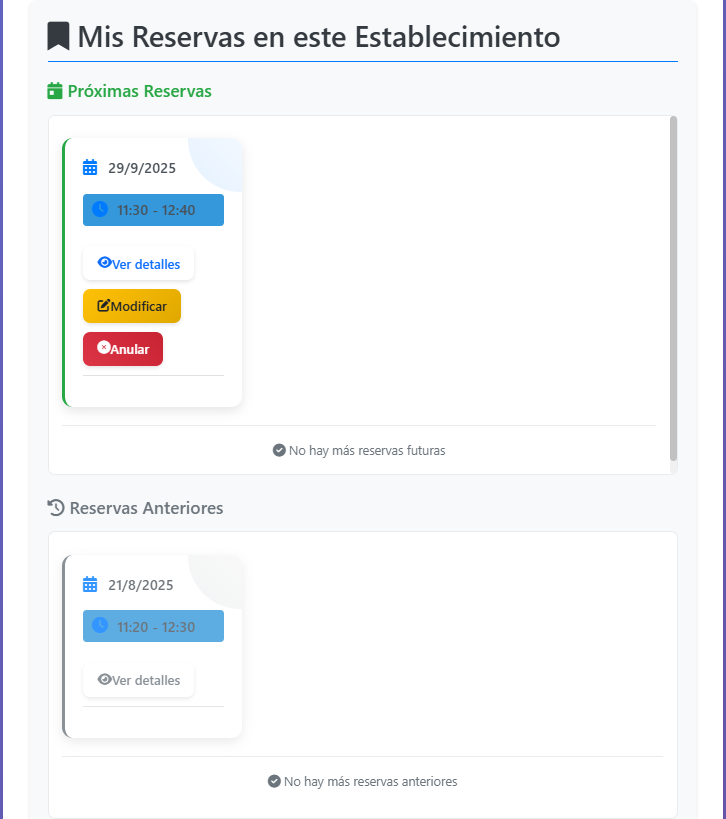
\includegraphics[width=0.5\linewidth]{reservapp_historial_reservas}
	\caption{Página con el historial de reservas.}
	\label{fig:reservapp_historial_reservas}
\end{figure}

\begin{enumerate}
   \item \textbf{Reservas futuras}:
   \begin{itemize}
      \item Lista de próximas reservas ordenadas por fecha.
	  \item Opciones para ver detalles, modificar o anular.
	  \item Información de convocatorias y usuarios invitados.
   \end{itemize}
   \item \textbf{Reservas pasadas}:
   \begin{itemize}
      \item Historial de reservas anteriores.
      \item Solo disponible la opción de ver detalles.
      \item Útil para consultar información de reuniones pasadas.
   \end{itemize}
   \item \textbf{Scroll infinito}:
   \begin{itemize}
      \item Las reservas se cargan dinámicamente al hacer scroll.
      \item Mejora el rendimiento con grandes cantidades de reservas.
   \end{itemize}
\end{enumerate}

\subsection{Gestión de Convocatorias}

\subsubsection{Crear Convocatoria}
Permite invitar a otros usuarios a una reserva y organizar reuniones, tal y como se ilustra en la figura~\ref{fig:reservapp_convocatoria}. Estos son los pasos a seguir:

\begin{figure}[H]
	\centering
		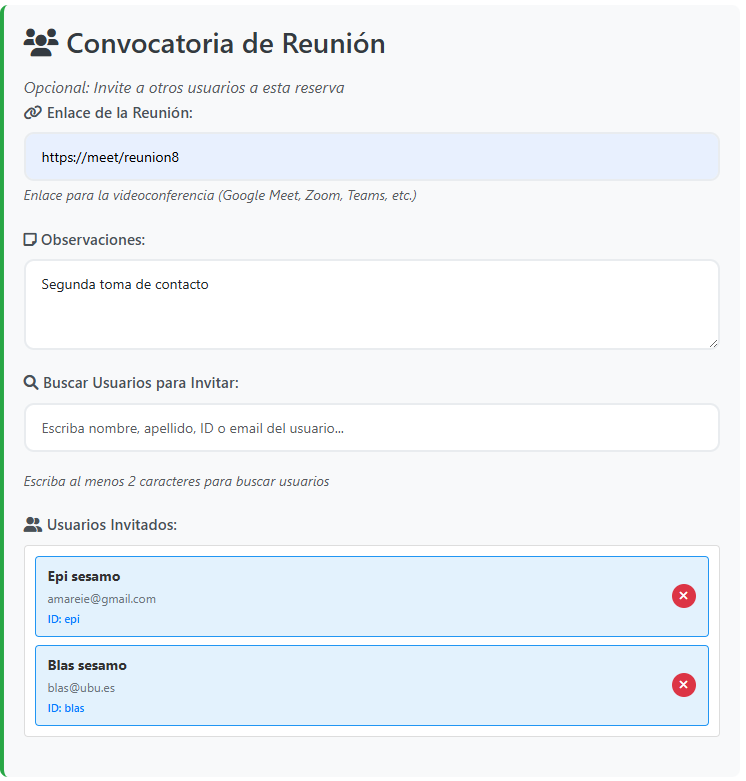
\includegraphics[width=0.5\linewidth]{reservapp_convocatoria}
	\caption{Sección de convocatoria vinculada a la reserva.}
	\label{fig:reservapp_convocatoria}
\end{figure}

\begin{enumerate}
   \item \textbf{Enlace de reunión}:
   \begin{itemize}
      \item URL de plataforma de videoconferencia.
      \item Formatos soportados: Google Meet, Zoom, Microsoft Teams, etc.
	  \item Campo opcional pero recomendado para reuniones virtuales.
   \end{itemize}
   \item \textbf{Observaciones}:
   \begin{itemize}
      \item Agenda de la reunión.
      \item Temas a tratar.
      \item Notas adicionales.
      \item Preparativos necesarios.
   \end{itemize}
   \item \textbf{Lista de invitados}:
   \begin{itemize}
      \item Búsqueda de usuarios por múltiples criterios.
      \item Selección múltiple de participantes.
      \item Vista previa de usuarios seleccionados.
   \end{itemize}
\end{enumerate}

\subsubsection{Gestionar Invitados}
Permite invitar a otros usuarios a una reserva y organizar reuniones, tal y como se ilustra en la figura~\ref{fig:reservapp_convocatoria}. Estos son los pasos a seguir:

\begin{enumerate}
   \item \textbf{Buscar usuarios}:
   \begin{itemize}
      \item Introducir al menos 2 caracteres en el campo de búsqueda.
      \item El sistema buscará por nombre, apellidos, ID de usuario o email.
	  \item Se mostrarán resultados en tiempo real.
   \end{itemize}
   \item \textbf{Seleccionar invitados}:
   \begin{itemize}
      \item Hacer clic en el usuario deseado de los resultados.
      \item El usuario se añadirá a la lista de invitados.
      \item Los usuarios ya seleccionados aparecen deshabilitados en futuras búsquedas.
   \end{itemize}
   \item \textbf{Gestionar lista de invitados}:
   \begin{itemize}
      \item Ver lista completa de usuarios invitados.
      \item Eliminar invitados haciendo clic en el botón ``X''.
      \item La lista se actualiza dinámicamente.
   \end{itemize}
\end{enumerate}

\subsubsection{Notificaciones de Convocatoria}
Permite invitar a otros usuarios a una reserva y organizar reuniones, tal y como se ilustra en la sección inferior de la figura~\ref{fig:reservapp_mis_reservas}. Estos son los pasos a seguir:

\begin{enumerate}
   \item \textbf{Creación de reserva con convocatoria}:
   \begin{itemize}
      \item Se envía email al creador de la reserva.
      \item Se envía email a todos los usuarios invitados.
	  \item Incluye detalles de fecha, hora, lugar y enlace de reunión.
   \end{itemize}
   \item \textbf{Modificación de reserva}:
   \begin{itemize}
      \item Notificación automática a todos los participantes.
      \item Incluye los cambios realizados.
   \end{itemize}
   \item \textbf{Anulación de reserva}:
   \begin{itemize}
      \item Notificación inmediata a todos los involucrados.
      \item Confirmación de cancelación.
   \end{itemize}
\end{enumerate}

\subsection{Gestión de Estbalecimientos}

\subsubsection{Explorar Establecimientos Disponibles}
Visualizar y solicitar acceso a nuevos establecimientos, tal y como se ilustra en la figura~\ref{fig:reservapp_asignacion_establecimiento}. Estos son los pasos a seguir:

\begin{figure}[H]
	\centering
		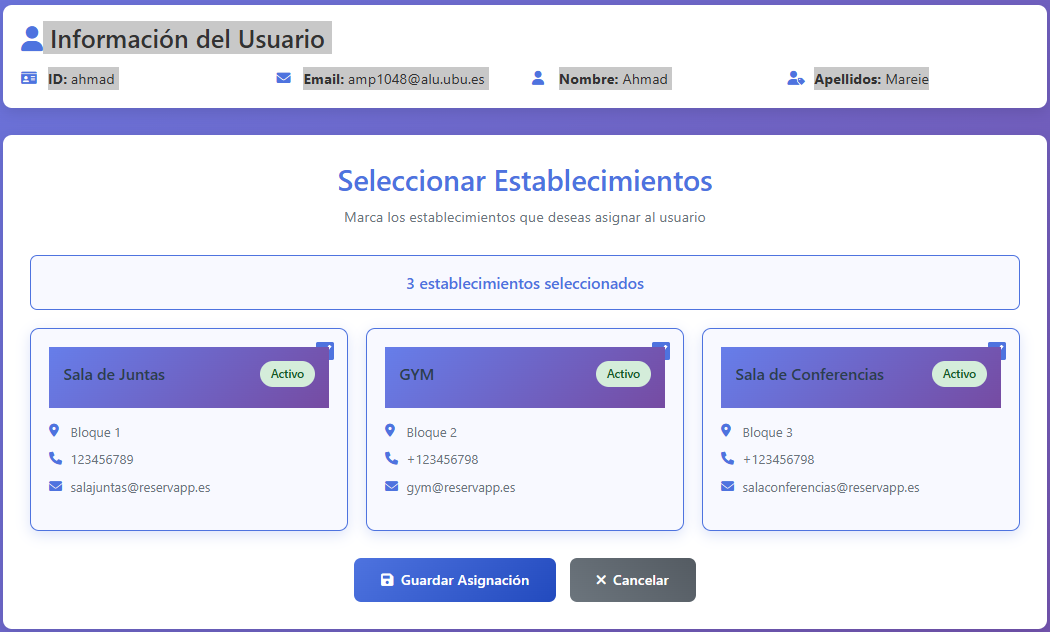
\includegraphics[width=0.5\linewidth]{reservapp_asignacion_establecimiento}
	\caption{Página de Establecimientos disponibles.}
	\label{fig:reservapp_asignacion_establecimiento}
\end{figure}

\begin{enumerate}
   \item \textbf{Acceder a asignación de establecimientos}:
   \begin{itemize}
      \item Desde el menú principal, hacer clic en ``Asignar Establecimientos''.
      \item O navegar a /establecimientos/asignar.
   \end{itemize}
   \item \textbf{Revisar establecimientos disponibles}:
   \begin{itemize}
      \item Lista completa de establecimientos del sistema.
      \item Información detallada de cada establecimiento.
	  \begin{itemize}
         \item Nombre y descripción.
         \item Tipo de establecimiento.
		 \item Capacidad y aforo.
		 \item Horarios de funcionamiento.
		 \item Información de contacto.
      \end{itemize}
   \end{itemize}
   \item \textbf{Solicitar asignación}:
   \begin{itemize}
      \item Seleccionar los establecimientos deseados mediante checkboxes.
      \item Hacer clic en ``Guardar Asignación''.
      \item El sistema procesará la solicitud.
   \end{itemize}
\end{enumerate}

\textbf{Nota}: La asignación puede requerir aprobación administrativa según la configuración del sistema.


\subsubsection{Gestionar Establecimientos Asignados}
Visualizar y solicitar acceso a nuevos establecimientos, tal y como se ilustra en la figura~\ref{fig:reservapp_asignacion_establecimiento}. Estos son los pasos a seguir:

\begin{enumerate}
   \item \textbf{Funcionalidades disponibles}:
   \begin{itemize}
      \item \textbf{Ver establecimientos asignados}.
      \begin{itemize}
         \item Lista de establecimientos a los que el usuario tiene acceso.
         \item Estado de cada establecimiento (activo/inactivo).
      \end{itemize}

      \item \textbf{Acceder a calendarios de reserva}.
      \begin{itemize}
         \item Hacer clic en cualquier establecimiento asignado.
         \item Acceso directo al sistema de reservas del establecimiento.
      \end{itemize}
   \end{itemize}
\end{enumerate}

\subsection{Gestión de Perfil Personal}

\subsubsection{Editar Información Personal}
Permite actualizar los datos personales del usuario, tal y como se ilustra en la figura~\ref{fig:reservapp_editar_perfil}. Estos son los pasos a seguir:

\begin{figure}[H]
	\centering
		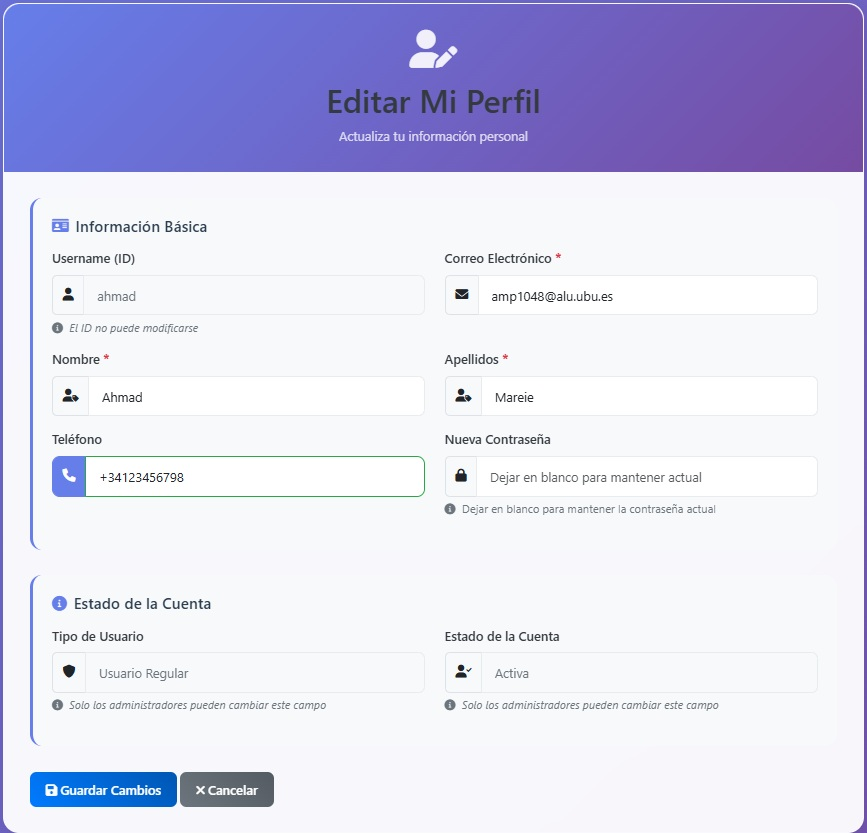
\includegraphics[width=0.5\linewidth]{reservapp_editar_perfil}
	\caption{Página de edición del perfil del usuario.}
	\label{fig:reservapp_editar_perfil}
\end{figure}

\begin{enumerate}
   \item \textbf{Acceder a edición de perfil}:
   \begin{itemize}
      \item Desde el menú principal, hacer clic en ``Editar Perfil''.
      \item O navegar a /perfiles.
   \end{itemize}
   \item \textbf{Modificar información}:
   \begin{itemize}
      \item \textbf{Datos personales}: Nombre, apellidos, teléfono.
      \item \textbf{Correo electrónico}: Cambiar email (debe ser único).
	  \item \textbf{Contraseña}: Actualizar contraseña (opcional).
   \end{itemize}
   \item \textbf{Guardar cambios}:
   \begin{itemize}
      \item Hacer clic en ``Guardar Cambios''.
      \item El sistema validará los datos y aplicará las modificaciones.
   \end{itemize}
\end{enumerate}

\textbf{Restricciones}:
\begin{itemize}
   \item El ID de usuario no se puede modificar.
   \item El correo electrónico debe ser único en el sistema.
   \item Los cambios de contraseña requieren confirmación.
\end{itemize}

\subsection{Funcionalidades Administrativas}
Nota: Las siguientes funcionalidades están disponibles únicamente para usuarios con rol de administrador.

\subsubsection{Gestión de Usuarios: Visualizar Usuarios}
Permite administrar todas las cuentas de usuario del sistema, tal y como se ilustra en la figura~\ref{fig:reservapp_gestion_usuarios}. Estos son los pasos a seguir:

\begin{figure}[H]
	\centering
		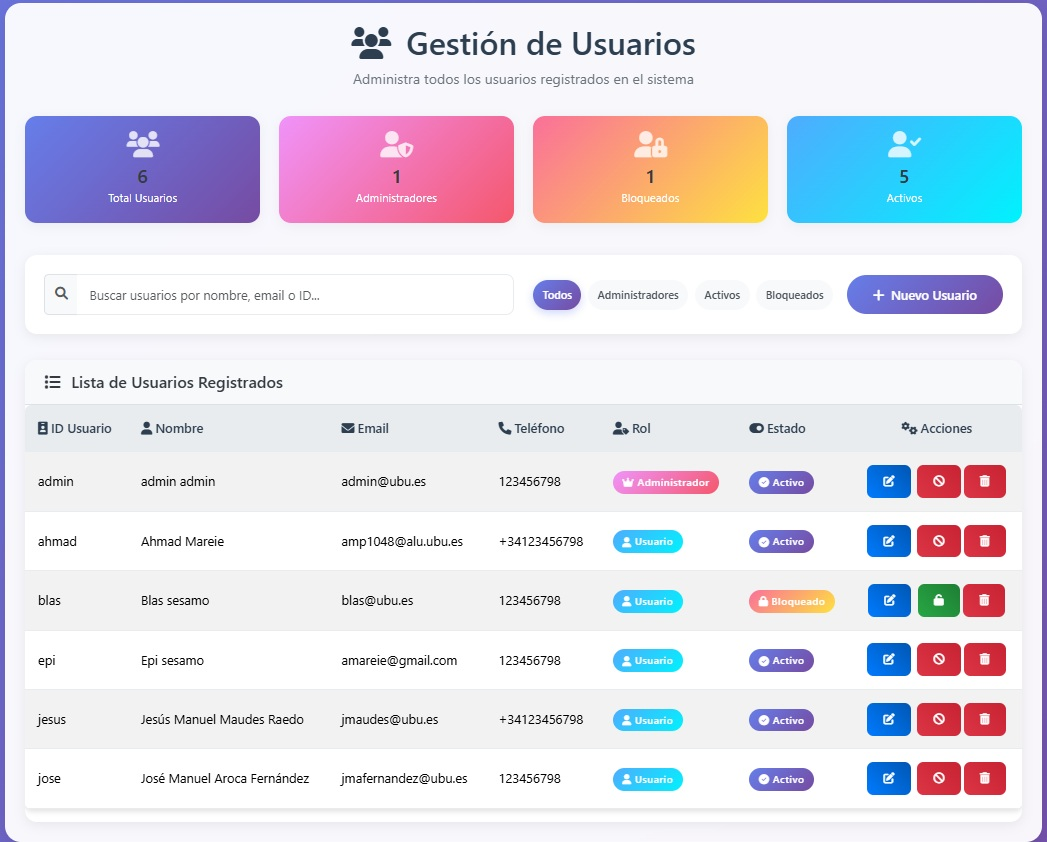
\includegraphics[width=0.5\linewidth]{reservapp_gestion_usuarios}
	\caption{Página de gestión de usuarios.}
	\label{fig:reservapp_gestion_usuarios}
\end{figure}

\begin{enumerate}
   \item \textbf{Acceder a gestión de usuarios}:
   \begin{itemize}
      \item Desde el menú principal, hacer clic en ``Gestión de Usuarios''.
      \item O navegar a /admin/usuarios.
   \end{itemize}
   \item \textbf{Revisar estadísticas del sistema}:
   \begin{itemize}
      \item \textbf{Total de usuarios}: Número total de cuentas registradas.
      \item \textbf{Administradores}: Cantidad de usuarios con privilegios administrativos.
	  \item \textbf{Usuarios bloqueados}: Cuentas deshabilitadas.
	  \item \textbf{Usuarios activos}: Cuentas habilitadas y funcionales.
   \end{itemize}
   \item \textbf{Utilizar herramientas de búsqueda y filtrado}:
   \begin{itemize}
      \item \textbf{Búsqueda}: Buscar por nombre, email o ID de usuario.
	  \item \textbf{Filtros}: Mostrar todos, solo administradores, solo activos, solo bloqueados.
      \item Los resultados se actualizan en tiempo real.
   \end{itemize}
\end{enumerate}

\subsubsection{Gestión de Usuarios: Crear nuevo usuario}
Permite crear un nuevo usuario en el sistema, tal y como se ilustra en la figura~\ref{fig:reservapp_nuevo_usuario}. Estos son los pasos a seguir:

\begin{figure}[H]
	\centering
		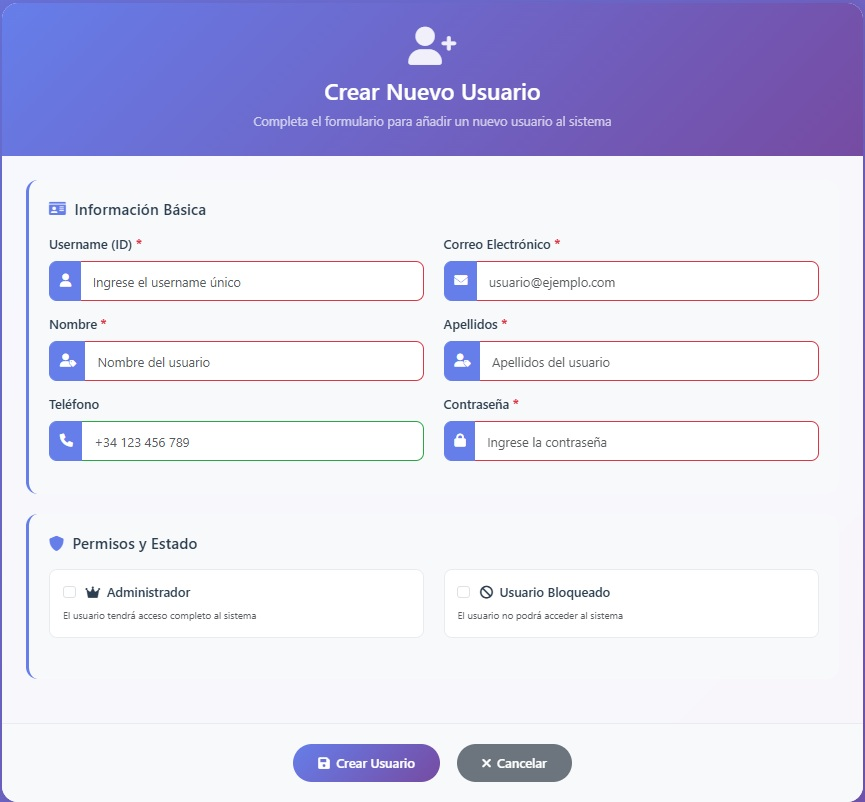
\includegraphics[width=0.5\linewidth]{reservapp_nuevo_usuario}
	\caption{Página con la ficha de usuario.}
	\label{fig:reservapp_nuevo_usuario}
\end{figure}

\begin{enumerate}
   \item \textbf{Iniciar creación}:
   \begin{itemize}
      \item Hacer clic en ``Nuevo Usuario''.
      \item Se abrirá el formulario de creación.
   \end{itemize}
   \item \textbf{Completar información del usuario}:
   \begin{itemize}
      \item \textbf{ID de Usuario}: Identificador único (3-10 caracteres alfanuméricos).
      \item \textbf{Datos personales}: Nombre, apellidos, teléfono.
	  \item \textbf{Correo electrónico}: Email único del usuario.
	  \item \textbf{Contraseña}: Contraseña inicial (obligatoria para nuevos usuarios).
	  \item \textbf{Rol}: Seleccionar si será administrador o usuario regular.
	  \item \textbf{Estado}: Definir si la cuenta estará activa o bloqueada.
   \end{itemize}
   \item \textbf{Guardar usuario}:
   \begin{itemize}
      \item Hacer clic en ``Guardar Usuario''.
	  \item El sistema validará los datos y creará la cuenta.
   \end{itemize}
\end{enumerate}

\subsubsection{Gestión de Usuarios: Editar usuario existente}
Permite modificar un usuario existente en el sistema, tal y como se ilustra en la figura~\ref{fig:reservapp_nuevo_usuario}. Estos son los pasos a seguir:

\begin{enumerate}
   \item \textbf{Seleccionar usuario}:
   \begin{itemize}
      \item Desde la lista de usuarios, hacer clic en el botón "Editar" (icono de lápiz).
   \end{itemize}
   \item \textbf{Modificar información}:
   \begin{itemize}
      \item \textbf{Datos personales}: Actualizar nombre, apellidos, teléfono.
      \item \textbf{Correo electrónico}: Cambiar email (debe seguir siendo único).
	  \item \textbf{Contraseña}: Dejar vacío para mantener la actual, o introducir nueva contraseña.
	  \item \textbf{Rol}: Cambiar entre usuario regular y administrador.
	  \item \textbf{Estado}: Modificar estado de bloqueo.
   \end{itemize}
   \item \textbf{Guardar usuario}:
   \begin{itemize}
      \item Hacer clic en ``Guardar Usuario''.
	  \item Los cambios se aplicarán inmediatamente.
   \end{itemize}
\end{enumerate}

\subsubsection{Gestión de Usuarios: Actualizar el Estado de Usuario}
Permite modificar el estado de un usuario existente en el sistema, tal y como se ilustra en la figura~\ref{fig:reservapp_nuevo_usuario}. Estos son los pasos a seguir:

\begin{enumerate}
   \item \textbf{Bloquear usuario}:
   \begin{enumerate}
      \item Hacer clic en el botón ``Bloquear'' (icono de prohibición) junto al usuario.
	  \item Confirmar la acción en el diálogo de confirmación.
	  \item El usuario no podrá acceder al sistema hasta ser desbloqueado
   \end{enumerate}
   \item \textbf{Desbloquear usuario}:
   \begin{enumerate}
      \item Hacer clic en el botón "Desbloquear" (icono de candado abierto) junto al usuario bloqueado.
      \item Confirmar la acción.
	  \item El usuario recuperará el acceso al sistema.
   \end{enumerate}
   \item \textbf{Eliminar usuario}:
   \begin{enumerate}
      \item Hacer clic en el botón "Eliminar" (icono de papelera) junto al usuario.
	  \item Confirmar la eliminación (acción irreversible).
	  \item Se eliminará la cuenta y todos sus datos asociados
   \end{enumerate}
\end{enumerate}

\textbf{Restricciones}:
\begin{itemize}
   \item Los administradores no pueden eliminar su propia cuenta.
   \item La eliminación de usuarios es irreversible.
   \item Se recomienda bloquear antes que eliminar para preservar el historial.
\end{itemize}

\subsubsection{Gestión de Establecimientos: Visualizar Establecimientos}
Permite administrar todos los establecimientos del sistema, tal y como se ilustra en la figura~\ref{fig:reservapp_gestion_establecimientos}. Estos son los pasos a seguir:

\begin{figure}[H]
	\centering
		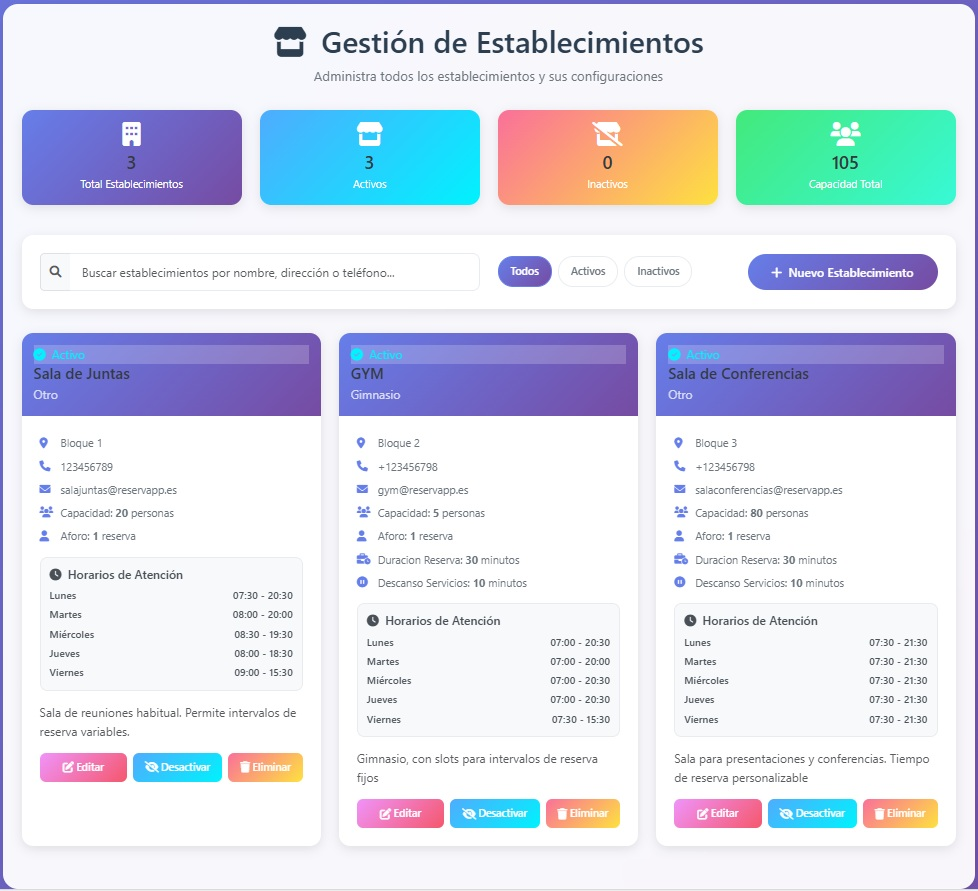
\includegraphics[width=0.5\linewidth]{reservapp_gestion_establecimientos}
	\caption{Página de Gestión de Establecimientos.}
	\label{fig:reservapp_gestion_establecimientos}
\end{figure}

\begin{enumerate}
   \item \textbf{Acceder a gestión de establecimientos}:
   \begin{itemize}
      \item Desde el menú principal, hacer clic en ``Gestión de Establecimientos''.
      \item O navegar a /admin/establecimientos.
   \end{itemize}
   \item \textbf{Revisar estadísticas}:
   \begin{itemize}
      \item \textbf{Total de establecimientos}: Número total registrado.
      \item \textbf{Establecimientos activos}: Disponibles para reservas.
	  \item \textbf{Establecimientos inactivos}: Temporalmente deshabilitados.
	  \item \textbf{Capacidad total}: Suma de capacidades de todos los establecimientos.
   \end{itemize}
   \item \textbf{Utilizar herramientas de búsqueda}:
   \begin{itemize}
      \item \textbf{Búsqueda}: Buscar por nombre, dirección o teléfono.
	  \item \textbf{Filtros}: Mostrar todos, solo activos, solo inactivos.
   \end{itemize}
\end{enumerate}

\subsubsection{Gestión de Establecimientos: Crear Nuevo Establecimiento}
Permite crear un nuevo establecimiento en el sistema, tal y como se ilustra en la figura~\ref{fig:reservapp_nuevo_establecimientos}. Estos son los pasos a seguir:

\begin{figure}[H]
	\centering
		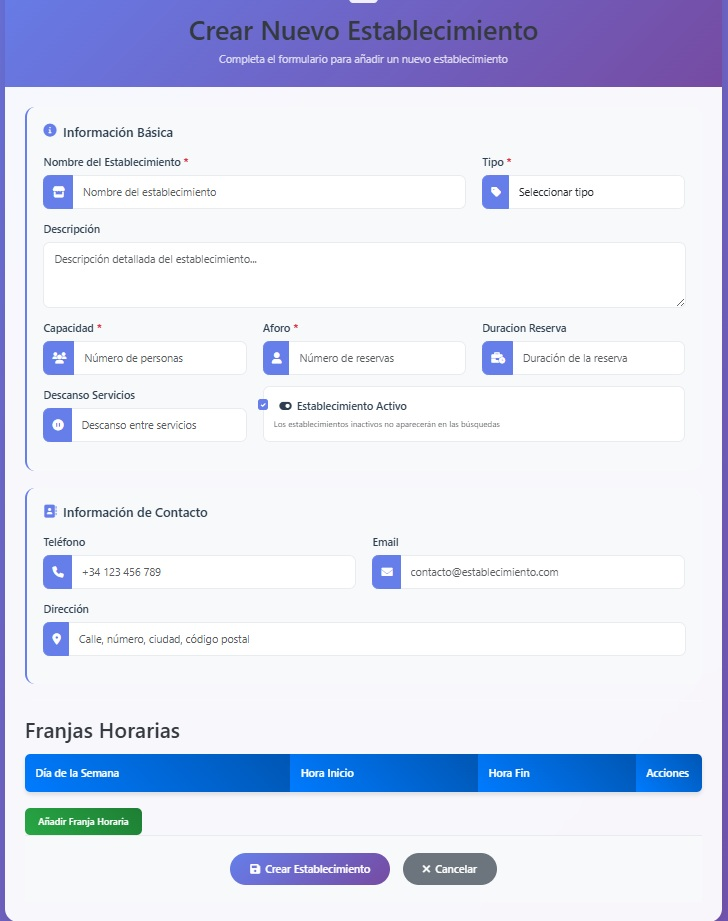
\includegraphics[width=0.5\linewidth]{reservapp_nuevo_establecimientos}
	\caption{Página de Nuevo Establecimiento.}
	\label{fig:reservapp_nuevo_establecimientos}
\end{figure}

\begin{enumerate}
   \item \textbf{Iniciar creación}:
   \begin{itemize}
      \item Hacer clic en ``Nuevo Establecimiento''.
   \end{itemize}
   \item \textbf{Completar información básica}:
   \begin{itemize}
      \item \textbf{Nombre}: Denominación del establecimiento (máximo 80 caracteres).
      \item \textbf{Descripción}: Descripción detallada (máximo 250 caracteres).
	  \item \textbf{Tipo}: Categoría del establecimiento.
	  \item \textbf{Dirección}: Ubicación física.
	  \item \textbf{Teléfono}: Número de contacto.
	  \item \textbf{Email}: Correo electrónico de contacto.
   \end{itemize}
   \item \textbf{Configurar parámetros operativos}:
   \begin{itemize}
      \item \textbf{Búsqueda}: Buscar por nombre, dirección o teléfono.
	  \item \textbf{Filtros}: Mostrar todos, solo activos, solo inactivos.
   \end{itemize}
   \item \textbf{Definir horarios de funcionamiento}:
   \begin{itemize}
      \item \textbf{Búsqueda}: Buscar por nombre, dirección o teléfono.
	  \item \textbf{Filtros}: Mostrar todos, solo activos, solo inactivos.
   \end{itemize}
   \item \textbf{Guardar establecimiento}:
   \begin{itemize}
      \item Hacer clic en ``Guardar Establecimiento''.
	  \item El establecimiento se creará en estado activo por defecto.
   \end{itemize}
\end{enumerate}

\subsubsection{Gestión de Establecimientos: Editar Establecimiento Existente}
Permite editar un establecimiento previamente creado en el sistema, tal y como se ilustra en la figura~\ref{fig:reservapp_nuevo_establecimientos}. Estos son los pasos a seguir:

\begin{enumerate}
   \item \textbf{Seleccionar establecimiento}:
   \begin{itemize}
      \item Hacer clic en ``Editar'' en la tarjeta del establecimiento deseado.
   \end{itemize}
   \item \textbf{Modificar información}:
   \begin{itemize}
      \item Actualizar cualquier campo de información básica.
      \item Ajustar parámetros operativos según necesidades.
	  \item Modificar horarios de funcionamiento.
   \end{itemize}
   \item \textbf{Guardar cambios}:
   \begin{itemize}
      \item Hacer clic en ``Guardar Cambios''.
	  \item Los cambios se aplicarán inmediatamente.
   \end{itemize}
\end{enumerate}

\subsubsection{Gestión de Establecimientos: Actualizar Estado de Establecimientos}
Permite actualizar el estado de un establecimiento previamente creado en el sistema, tal y como se ilustra en la figura~\ref{fig:reservapp_gestion_establecimientos}. Estos son los pasos a seguir:

\begin{itemize}
   \item \textbf{Activar/Desactivar establecimiento}:
   \begin{enumerate}
      \item Hacer clic en ``Activar'' o ``Desactivar'' según el estado actual.
	  \item Confirmar la acción
	  \item Los establecimientos inactivos no estarán disponibles para nuevas reservas
   \end{enumerate}
   \item \textbf{Eliminar establecimiento}:
   \begin{enumerate}
      \item Hacer clic en ``Eliminar''.
      \item Confirmar la eliminación (acción irreversible).
	  \item Se eliminará el establecimiento y todas sus reservas asociadas.
   \end{enumerate}
\end{itemize}

\subsubsection{Gestión de Perfiles: Visualizar Establecimientos}
Permite administrar todos los perfiles del sistema, tal y como se ilustra en la figura~\ref{fig:reservapp_gestion_perfiles}. Estos son los pasos a seguir:

\begin{figure}[H]
	\centering
		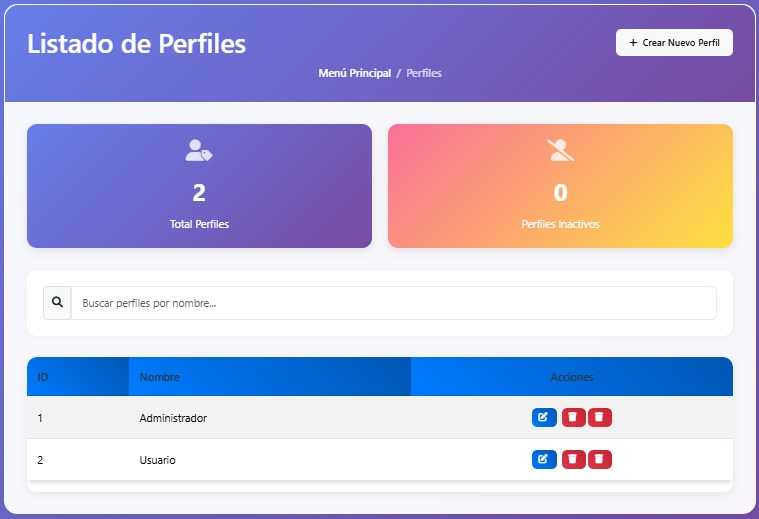
\includegraphics[width=0.5\linewidth]{reservapp_gestion_perfiles}
	\caption{Página de Gestión de Perfiles.}
	\label{fig:reservapp_gestion_perfiles}
\end{figure}

\begin{enumerate}
   \item \textbf{Acceder a gestión de perfiles}:
   \begin{itemize}
      \item Desde el menú principal, hacer clic en ``Gestión de Perfiles''.
      \item O navegar a /admin/perfiles.
   \end{itemize}
   \item \textbf{Revisar perfiles existentes}:
   \begin{itemize}
      \item Lista de todos los perfiles configurados.
      \item Información de cada perfil y sus características.
   \end{itemize}
\end{enumerate}

\subsubsection{Gestión de Perfiles: Crear Nuevo Perfil}
Permite crear un nuevo perfil en el sistema, tal y como se ilustra en la figura~\ref{fig:reservapp_nuevo_perfil}. Estos son los pasos a seguir:

\begin{figure}[H]
	\centering
		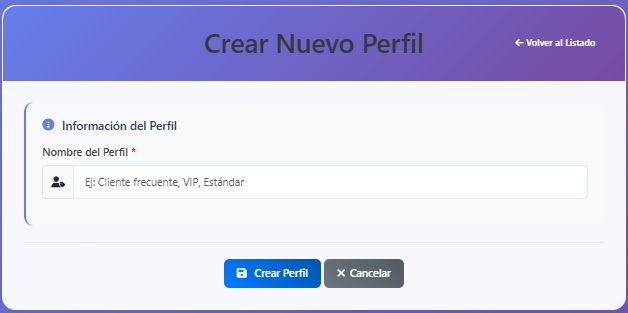
\includegraphics[width=0.5\linewidth]{reservapp_nuevo_perfil}
	\caption{Página de Nuevo Perfil.}
	\label{fig:reservapp_nuevo_perfil}
\end{figure}

\begin{enumerate}
   \item \textbf{Iniciar creación}:
   \begin{itemize}
      \item Hacer clic en ``Nuevo Perfil''.
   \end{itemize}
   \item \textbf{Completar información básica}:
   \begin{itemize}
      \item \textbf{Nombre}: Denominación del perfil.
      \item \textbf{Descripción}: Descripción de las funcionalidades del perfil.
   \end{itemize}
   \item \textbf{Guardar perfil}:
   \begin{itemize}
      \item Hacer clic en ``Guardar Perfil''.
   \end{itemize}
\end{enumerate}

\subsubsection{Gestión de Perfiles: Editar o eliminar Perfiles}
Permite crear un nuevo perfil en el sistema, tal y como se ilustra en la figura~\ref{fig:reservapp_gestion_perfiles}. Estos son los pasos a seguir:

\begin{itemize}
   \item \textbf{Editar perfil}:
   \begin{enumerate}
      \item Hacer clic en ``Editar'' junto al perfil deseado.
	  \item Modificar la información necesaria.
	  \item Guardar los cambios.
   \end{enumerate}
   \item \textbf{Eliminar perfil}:
   \begin{enumerate}
      \item Hacer clic en ``Eliminar'' junto al perfil.
      \item Confirmar la eliminación.
   \end{enumerate}
\end{itemize}

\subsubsection{Supervisión de Reservas: Vista General de Reservas}
Permite monitorear y gestionar todas las reservas del sistema., tal y como se ilustra en la figura~\ref{fig:reservapp_gestion_reservas}. Estos son los pasos a seguir:

\begin{figure}[H]
	\centering
		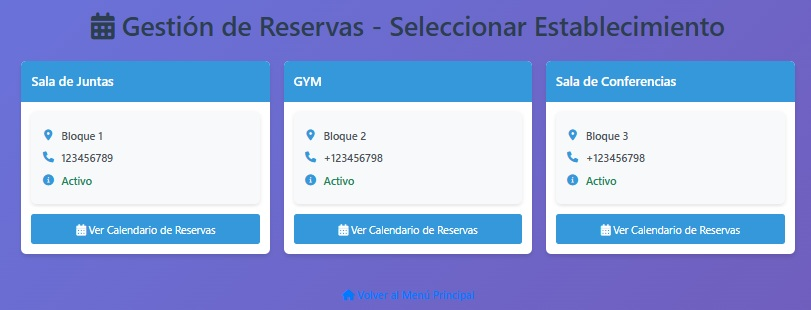
\includegraphics[width=0.5\linewidth]{reservapp_gestion_reservas}
	\caption{Vista previa de los establecimientos para ver las reservas.}
	\label{fig:reservapp_gestion_reservas}
\end{figure}

\begin{enumerate}
   \item \textbf{Acceder a gestión de reservas}:
   \begin{itemize}
      \item Desde el menú principal, hacer clic en ``Gestión de Reservas''.
      \item O navegar a /admin/reservas.
   \end{itemize}
   \item \textbf{Seleccionar establecimiento}:
   \begin{itemize}
      \item Elegir el establecimiento a supervisar de la lista disponible.
   \end{itemize}
\end{enumerate}

\subsubsection{Supervisión de Reservas: Calendario Mensual de Reservas}
Permite ver el calendario mensual de las reservas que tiene un establecimiento, tal y como se ilustra en la figura~\ref{fig:reservapp_calendario_reservas}. Estos son los pasos a seguir:

\begin{figure}[H]
	\centering
		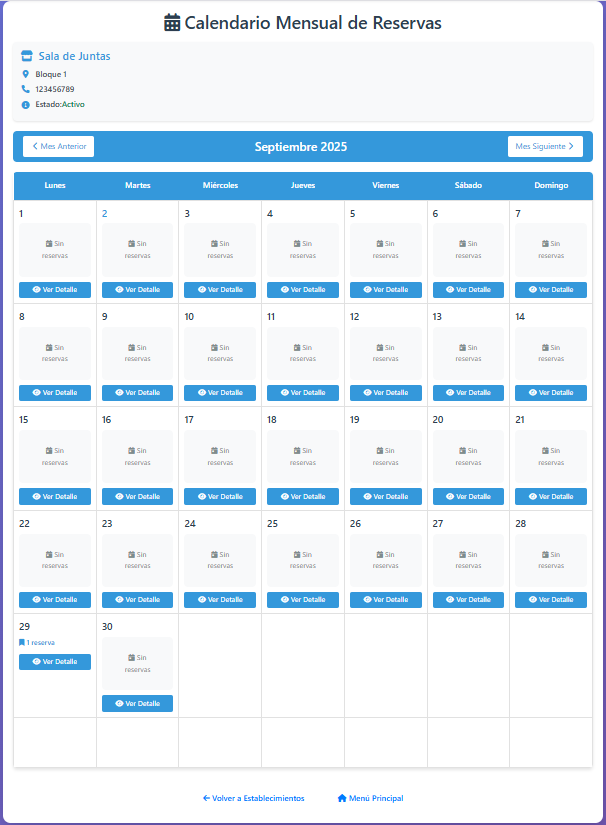
\includegraphics[width=0.5\linewidth]{reservapp_calendario_reservas}
	\caption{Calendario mensual de reservas de un establecimiento.}
	\label{fig:reservapp_calendario_reservas}
\end{figure}

\begin{enumerate}
   \item \textbf{Navegación temporal}:
   \begin{itemize}
      \item Cambiar entre meses y años usando los controles de navegación.
	  \item Vista de calendario mensual con todas las reservas.
   \end{itemize}
   \item \textbf{Información por día}:
   \begin{itemize}
      \item Cada día muestra el número de reservas programadas.
      \item Colores diferentes indican la densidad de reservas.
   \end{itemize}
   \item \textbf{Acceso a detalles diarios}:
   \begin{itemize}
      \item Hacer clic en cualquier día para ver las reservas específicas.
	  \item Vista detallada de todas las reservas del día seleccionado
   \end{itemize}
\end{enumerate}

\subsubsection{Supervisión de Reservas: Detalle de Reservas Diarias}
Permite ver el detalle de una reserva en concreto, tal y como se ilustra en la figura~\ref{fig:reservapp_detalle_reservas}. Estos son los pasos a seguir:

\begin{figure}[H]
	\centering
		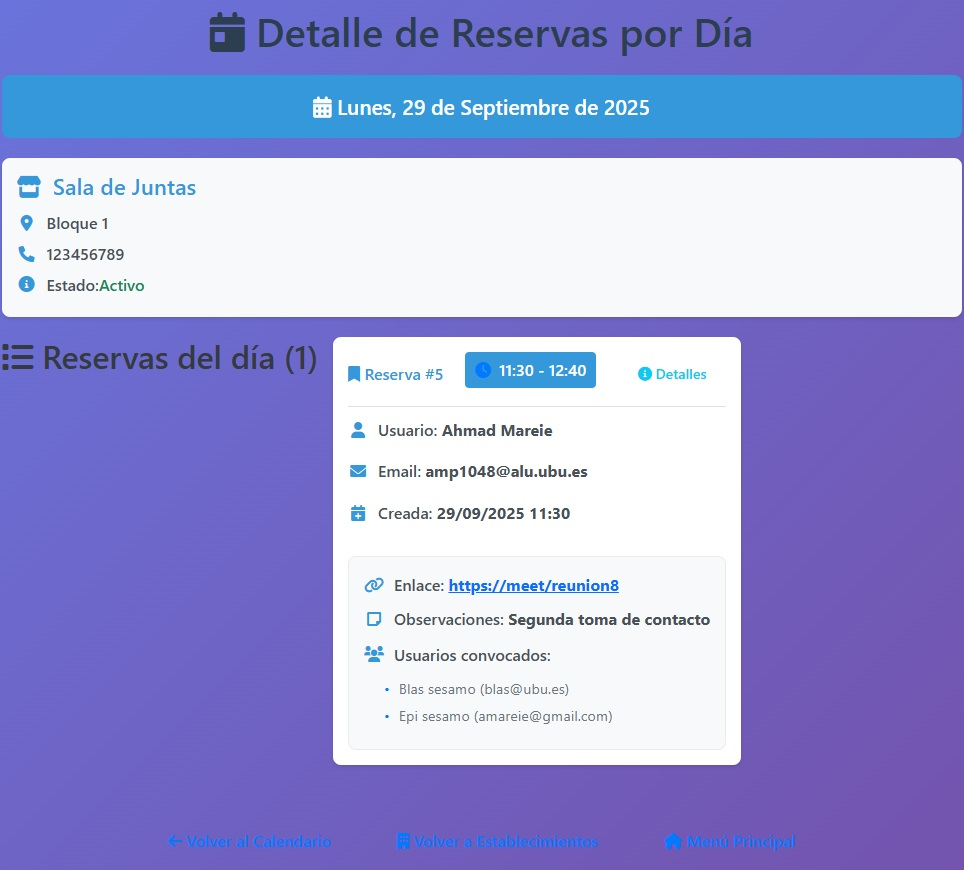
\includegraphics[width=0.5\linewidth]{reservapp_detalle_reservas}
	\caption{Detalle de una reserva particular.}
	\label{fig:reservapp_detalle_reservas}
\end{figure}

\begin{enumerate}
   \item \textbf{Lista de reservas del día}:
   \begin{itemize}
      \item Hora de cada reserva.
      \item Usuario que realizó la reserva.
      \item Información de contacto.
      \item Detalles de la convocatoria (si existe).
   \end{itemize}
   \item \textbf{Gestión de reservas}:
   \begin{itemize}
      \item Visualización completa de todas las reservas.
      \item Información de usuarios convocados.
      \item Enlaces de reunión y observaciones.
   \end{itemize}
\end{enumerate}

\subsection{Resolución de problemas comunes}

\begin{itemize}
   \item \textbf{Problemas de Acceso}:
   \begin{itemize}
      \item No puedo iniciar sesión:
      \begin{itemize}
         \item Verificar que el ID de usuario y contraseña sean correctos.
         \item Comprobar que la cuenta no esté bloqueada.
         \item Contactar con el administrador si persiste el problema.
      \end{itemize}
      \item He olvidado mi contraseña:
      \begin{itemize}
         \item Contactar con el administrador del sistema para restablecer la contraseña.
         \item El administrador puede asignar una contraseña temporal.
      \end{itemize}
   \end{itemize}

   \item \textbf{Problemas con Reservas}:
   \begin{itemize}
      \item No puedo crear una reserva:
      \begin{itemize}
         \item Verificar que el establecimiento esté activo.
         \item Comprobar que la fecha y hora estén dentro de los horarios de apertura.
         \item Verificar que no se haya alcanzado el aforo máximo.
         \item Asegurarse de que la hora de fin sea posterior a la hora de inicio.
      \end{itemize}
      \item No veo mis reservas:
      \begin{itemize}
         \item Verificar que esté accediendo al establecimiento correcto.
         \item Comprobar que tenga permisos para el establecimiento.
         \item Las reservas muy antiguas pueden no mostrarse por defecto.
      \end{itemize}
      \item Error al modificar una reserva:
      \begin{itemize}
         \item Solo se pueden modificar reservas futuras.
         \item Verificar que sea el propietario de la reserva.
         \item Comprobar la disponibilidad del nuevo horario solicitado.
      \end{itemize}
   \end{itemize}

   \item \textbf{Problemas con Convocatorias}:
   \begin{itemize}
      \item Los usuarios invitados no reciben emails:
      \begin{itemize}
         \item Verificar que las direcciones de email sean correctas.
         \item Comprobar las carpetas de spam/correo no deseado.
         \item Contactar con el administrador para verificar la configuración del servidor de correo.
      \end{itemize}
      \item No puedo encontrar usuarios para invitar:
      \begin{itemize}
         \item Verificar que esté escribiendo al menos 2 caracteres.
         \item Comprobar que los usuarios existan en el sistema.
         \item Los usuarios bloqueados pueden no aparecer en los resultados.
      \end{itemize}
   \end{itemize}

   \item \textbf{Problemas de Rendimiento}:
   \begin{itemize}
      \item La aplicación carga lentamente:
      \begin{itemize}
         \item Verificar la conexión a internet.
         \item Limpiar la caché del navegador.
         \item Contactar con el administrador si el problema persiste.
      \end{itemize}
      \item Los horarios no se cargan:
      \begin{itemize}
         \item Verificar que haya seleccionado una fecha válida.
         \item Comprobar que el establecimiento tenga horarios configurados.
         \item Refrescar la página si el problema persiste.
      \end{itemize}
   \end{itemize}
\end{itemize}
